\documentclass[titlepage]{article}
\usepackage[left=15mm,right=15mm,top=1in,bottom=1in]{geometry}
\usepackage{framed}
\usepackage{caption}
\usepackage{imakeidx}
\usepackage{graphicx}
\usepackage{hyperref}
\usepackage{array}

\newcolumntype{C}[1]{>{\centering\arraybackslash} m{#1cm}}
\graphicspath{{./img/}}

\makeindex

\title{\textbf{\Huge{Offer Acceptance Prediction Tool}}\\[20mm]Advanced Optimization Laboratory\\~\\\textbf{\Huge{High-Level Software Design}}}
\author{Eric Le Fort}
 
\begin{document}
\maketitle
\tableofcontents
~\\[15mm]
\listoftables
\listoffigures


\vfill
\begin{table}[!htbp]
\centering
\begin{tabular}{| C{3} | C{2} | C{10} |}\hline
	Date			&Revision \#	&Comments\\\hline
	11-JUN-2017		&0				&- Initial document creation\\\hline
	27-OCT-2017		&1				&- Document modified to better reflect state of the code.\\\hline	
\end{tabular}
\caption{Revision History}
\label{tab:RevisionHistory}
\end{table}
\newpage
 
\section{Introduction}
This document aims to provide a high-level design overview of the offer acceptance prediction tool for AdvOL. In particular it will cover topics such as the architectural design, plans for the design process of the machine learning and dimensionality reduction algorithms, and the use cases this system must handle.
\subsection{System Description}
This system is intended to predict the number of accepted offers given an acceptance average in order to better inform the Dean's Office in their decision. This goal will be achieved by gathering information regarding applicant data from current and past years. This applicant information will then be fed into the trained model in order to derive a probability of that applicant accepting the offer. Several types of models will be experimented with in order to compare their effectiveness.\\~\\
The following block diagram will illustrate how this system will be constructed.\vfill
\begin{center}
	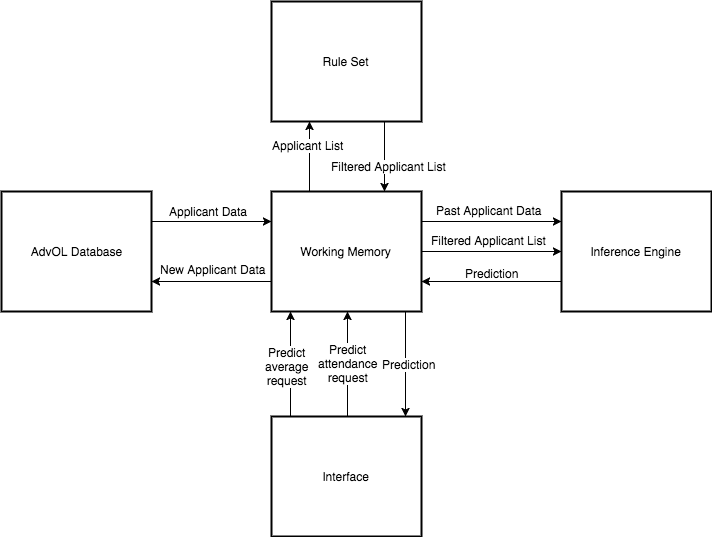
\includegraphics[width=0.9\textwidth]{AdvolBlockDiagram.png}
\captionof{figure}{System Block Diagram}
\label{fig:block diagram}
\end{center}
\subsection{Overview}
This document has three sections not including this one. Each section contains either design diagrams or further explanations to further describe the architecture of this system and is intended to prepare the development team to implement the design.\\
\begin{itemize}
	\item \textbf{Architectural Design}: This section describes the chosen system architecture. It will also discuss which components are likely to change in future versions.\\
	\item \textbf{Machine Learning Design}: This section describes how dimensionality reduction and algorithmic selection will be performed.\\
	\item \textbf{Use Cases}: This section describes possible interactions this system must handle as well as the intended results of those interactions.\\
\end{itemize}
\subsection{Naming Conventions \& Definitions}
All necessary acronyms, abbreviations, and definitions can be found in the \textit{Requirements} document for this system.



\section{Architectural Design}
This section discusses the architectural design of this system. Importantly, it also discusses components that are likely to change in future versions.
\subsection{System Architecture}
This system will implement a \textit{Rule-Based} architecture which is well-suited to machine learning problems. This style breaks the system down into four types of modules: an interface, a rule set, working memory, and an inference engine. The interface is where the system will receive its input and display its output. The rule set is a particular sort of knowledge base which constrains the acceptable results. The working memory is temporary memory used by the module designed to provide quick access to the relevant context. Lastly, the inference engine is what ties the system together. Its job is to apply the rules and, using the working memory as a resource, generate the appropriate result to send as output.\\~\\
In the case of this system, the breakdown of these modules into these types will be as follows:\\
\begin{itemize}
	\item Interface
	\begin{itemize}
		\item[-] Input: A selection of whether the input is an acceptance average or a target enrolment.
		\item[-] Input: The value of the acceptance average or target enrolment.
		\item[-] Output: The projected acceptance average or enrolment.
		\item[-] A connection to populate the database using raw data files.
		\item[-] A connection to read data from the database.
	\end{itemize}
	\item Rule Set
	\begin{itemize}
		\item[-] Hard-coded filtering rules (e.g. an absolute minimum grade in a certain course)
	\end{itemize}
\end{itemize}
\newpage
\begin{itemize}
	\item Working Memory
	\begin{itemize} 
		\item[-] Applicant data from all years as well as known previous results
		\item[-] The trained models
	\end{itemize}
	\item Inference Engine
	\begin{itemize}
		\item[-] The training algorithm
		\item[-] The algorithm to apply the model to an applicant to gauge the likelihood they accept an offer
	\end{itemize}
\end{itemize}
\subsection{Likely Changes}
The nature of this system necessitates certain components are likely to change during its lifetime. For example, both the dimensionality reduction algorithm and machine learning algorithm will have various alternatives to be tested. A final version will not be selected until near the end of development of version 1. Another likely change involves the data itself. From year to year, features are sometimes added, removed, or modified and so the system should be designed to handle these changes as gracefully as possible.



\section{Machine Learning Design}
This section will discuss high-level design choices pertaining to the machine learning aspects of this system. In particular it will describe the process for reducing the problem's dimensionality as well as the experimentation that will be performed in order to empirically choose an optimal algorithm for the specific problem.
\newpage
\subsection{Dimensionality Reduction}
An essential factor to the success of this project involves the selection of meaningful features. The following list holds the features which are available.\\
\begin{table}[!htbp]
\centering
\begin{tabular}{| C{4} | C{10} |}\hline
	\textbf{Feature}				&\textbf{Description}\\\hline
	School ID						&Ontario Secondary School number of the applicant's school.\\\hline
	School Board					&Ontario Secondary School board of the applicant's school.\\\hline
	School Region					&County/region of school of the applicant's school.\\\hline
	Sex								&Gender of applicant.\\\hline
	Birthday						&Applicant's birthday.\\\hline
	Location of Residence			&The country, province, county, and postal code of the applicant's residence.\\\hline
	Immigration Status				&This applicant's immigration status.\\\hline
	Citizenship						&The citizenship country and region of this applicant.\\\hline
	Mother Tongue					&The applicant's native tongue.\\\hline
	Applicant Type					&\\\hline%TODO what is this?
	Confirmed Details				&The confirmed university, program group, program, program year level, enrolment term, and OUAC choice preference of this applicant.\\\hline
	Choice Ranking					&This applicant's OUAC confirmed choice preference.\\\hline
	Registered Details				&The registered university, program group, program, program year level, enrolment term, and OUAC choice preference of this applicant.\\\hline
	Senior Level Courses Data		&The course info for this applicant's 12 senior level courses including course codes, course credits, and final marks.\\\hline
	Senior Level Courses Summary	&The number of senior level courses this applicant took and their total senior level credits.\\\hline
	Years in Secondary				&The number of years this applicant was in secondary school.\\\hline
	Average 1						&The average of the applicant's best 6 senior level course finals from this year.\\\hline
	Average 2						&The average of the applicant's best 6 senior level course finals from all years.\\\hline
	More than 20					&A flag indicating the applicant has more than 20 choices.\\\hline
	Application Choice Data			&The applicant's application preferences for up to 20 choices including the ranking of each choice. Each choice also contains: the university, program group, program, full-time or part-time, enrolment term, major interest, co-op or not co-op, and the year level.\\\hline
	Offer Data						&The program group, program, enrolment term, and year level offered to this applicant.\\\hline
	Confirmed Indicator				&Whether the applicant has confirmed their offer.\\\hline
	Registered Indicator			&Whether the applicant has registered.\\\hline
	Sequence Number					&The sequence number of this application.\\\hline
\end{tabular}
\caption{Applicant Feature Set}
\label{tab:ApplicantFeatureSet}
\end{table}~\\[6mm]
Selecting the features which correlate closest to the predictions we are trying to make will be done by performing Kernel Principal Component Analysis (KPCA). This algorithm automatically captures the maximum amount of variance within the data using nonlinear combinations of features while minimizing the number of components necessary.
\subsection{Model Training}
The model will be trained using the transformed features from the KPCA module. All but the most recent year's data will be used for training. This technique was chosen in order to best emulate the real-world operation of this system -- new data will be available once per year and only previous years' data will be available. After fitting the model to the data, it will be able to predict the likelihood of an applicant accepting an offer of admission.
\subsection{Testing}
Testing will be performed using the data of the most recent finalized year. Using the chosen acceptance average, we can see how accurate the model would have been at predicting offer acceptance.
\subsection{Algorithm Selection}
The final selection of the learning algorithm will be made after experimenting with various potential candidate algorithms which will be scored based on their performance and accuracy.\\~\\
Candidates that are likely to perform well include K-Nearest Neighbour, Random Forest, Naive Bayes, or some form of neural network. Various other algorithms such as Support Vector Machines, logistic regression or simple decision trees will also be tested for completeness.



\section{Use Cases}
This section will go over the various use cases that this system is expected to handle. For each use case, a description of the desired results and how the system will handle operating to achieve those results will be provided.
\subsection{Setup Process}
Upon startup, the system must perform certain tasks. For one, past model information and saved prediction results must be loaded from saved data. If it is the first time the system is running, it must train the model. Once this is done it must initialize a thread to perform background predictions while the system is idle.
\subsection{Shutdown Process}
Upon shutdown, the system must write certain state data to storage such as prediction results, KPCA results, and trained models. Further, the system must signal all background threads to terminate.
\subsection{Access Request}
Every time a user tries to access the system they must be authenticated. A user will be denied access if they do not pass the necessary authentication steps. Due to concerns relating to data privacy, all access to this system will be required to originate from a specific VPN. This way, the origin of the request can be authenticated more reliably.
\subsection{Model Update}
Model updates will take place whenever a new year's data is available. This will involve performing both dimensionality reduction and model training.
\subsection{Acceptance Average Request}
The user will provide a desired quantity of accepted offers. The system will predict the acceptance average resulting in that quantity of accepted offers. This type of prediction will only be front-facing. Internally, various expected number of acceptances requests will be performed in order to find the average which most closely resembles the target quantity of accepted offers.
\subsection{Predicted Acceptances Request}
The user will provide an acceptance average. The system will predict the quantity of accepted offers by predicting the likelihood of each applicant accepting their offer.
\end{document}





